\documentclass[12pt]{article}

% JASA necessities --------
% NOTE: To produce blinded version, replace "1" with "0" below.
\newcommand{\blind}{1}
\pdfminorversion=4
% DON'T change margins - should be 1 inch all around.
% Daniel: This stuff seems not to have that effect despite the JASA
% template's claim (the bottom margin is huge)
% \addtolength{\oddsidemargin}{-.5in}%
% \addtolength{\evensidemargin}{-.5in}%
% \addtolength{\textwidth}{1in}%
% \addtolength{\textheight}{-.3in}%
% \addtolength{\topmargin}{-.8in}%
\usepackage[margin=1in]{geometry} % use this instead

\def\spacingset#1{\renewcommand{\baselinestretch}%
{#1}\small\normalsize} \spacingset{1}
% End JASA stuff --------------


\usepackage[letterpaper=true,colorlinks=true,pdfpagemode=none,urlcolor=blue,linkcolor=blue,citecolor=blue,pdfstartview=FitH]{hyperref}
\usepackage{amsmath,amsfonts,amssymb}
\usepackage{graphicx}
\usepackage{color}
\usepackage[round,sort&compress]{natbib}
\usepackage{algorithm,algorithmic}
\def\algorithmautorefname{Algorithm}


\usepackage{pgf}
\usepackage{tikz}
\usetikzlibrary{fit,arrows,automata}					% fitting shapes to coordinates
\usetikzlibrary{backgrounds}
%\usepackage{autonum}


% Bibliography

\renewcommand*{\figureautorefname}{Figure}%
\renewcommand*{\tableautorefname}{Table}%
\renewcommand*{\partautorefname}{Part}%
\renewcommand*{\chapterautorefname}{Chapter}%
\renewcommand*{\sectionautorefname}{Section}%
\renewcommand*{\subsectionautorefname}{Section}%
\renewcommand*{\subsubsectionautorefname}{Section}% 


%\graphicspath{{../PLS/plsPlotsv2/}}
%\renewcommand{\includegraphics}[2][]{}

% Number only ref'ed equations
\usepackage{mathtools}
%\mathtoolsset{showonlyrefs,showmanualtags}

\newcommand{\attn}[1]{\textcolor{red}{Note: #1}}
\newcommand{\norm}[1]{\left\lVert #1 \right\rVert}

\begin{document}

\if1\blind
{
\title{Markov-switching State Space Models for Uncovering Musical Interpretation}
\author{Daniel J. McDonald\thanks{
    The authors gratefully acknowledge
    support from the National Science Foundation (grants DMS-1407439
    and DMS-1753171).}\hspace{.2cm}\\ 
    Department of Statistics, Indiana University\\
    and\\
    Michael McBride\\
    Department of Statistics, Indiana University}
\maketitle
} \fi

% For JASA blinding------------
\if0\blind
{
  \bigskip
  \bigskip
  \bigskip
  \begin{center}
    {\LARGE\bf Markov-switching State Space Models for Uncovering Musical Interpretation}
\end{center}
  \medskip
} \fi
% end blinding ---------------

\bigskip
\begin{abstract}
For concertgoers, musical interpretation is the most important factor
in determining whether or not we enjoy a classical performance. Every
performance includes mistakes---intonation issues, a lost note, an
unpleasant sound---but these are all easily forgotten (or unnoticed) when a performer
engages her audience, imbuing a piece with novel emotional content
beyond the vague instructions inscribed on the printed page. While music teachers use
imagery or heuristic guidelines to motivate interpretive decisions, combining these
vague instructions to create a convincing performance remains the domain
of the performer, subject to the whims of the moment, technical
fluency, and taste. In this
research, we use data from the CHARM Mazurka Project---forty-six professional
recordings of Chopin's Mazurka Op.\ 63 No.\ 3 by consumate artists---with the goal of
elucidating musically interpretable performance decisions. Using information on the
tempo the recordings, we apply functional data
analysis techniques enriched with prior information gained from music
theory to discover relevant features and perform hierarchical
clustering. The resulting clusters suggest methods for informing music
instruction, discovering listening preferences, and analyzing performances.

%The text of your abstract. 200 or fewer words. At 172 currently
\end{abstract}

\noindent%
{\it Keywords:}  keyword1; keyword2; 
\vfill

%\newpage

\spacingset{1.45} % DON'T change the spacing!

% \tableofcontents










\section{Introduction}
\label{sec:introduction}

\attn{See \href {http://amstat.tfjournals.com/asa-style-guide/}{here}
  for the style guide (detailed) and
  \href{https://www.tandfonline.com/action/authorSubmission?journalCode=uasa20&page=instructions}{here}
  for the author instructions.}

In recent years, statistical analysis of recorded music has
become more and more important to academics and industry. Online
music services like Pandora, Last.fm, Spotify, and others rely on
recommendation systems to suggest potentially interesting or related
songs to listeners. In 2011, the KDD Cup challenged academic computer
scientists and statisticians to identify user tastes in music with the
\href{http://labrosa.ee.columbia.edu/millionsong/}{Yahoo! Million
  Song Dataset} (see \citet{DrorKoenigstein2012} for details of the
competition). Pandora, through its proprietary
\href{https://www.pandora.com/about/mgp}{Music Genome Project}, uses
trained musicologists to assign new songs a vector of trait
expressions (consisting of up to 500 `genes' depending on the genre)
which can then be used to measure similarity with other
songs. However, most of this work has focused on the analysis of more popular
and more profitable genres of music---pop, rock, country---as opposed
to classical music. 

Western classical music, classical music for short, is a subcategory
of music whose boundaries are occasionally difficult to define. But
the distinction is of great importance when it comes to the analysis
which we undertake here. Leonard Bernstein, the great composer,
conductor and pianist, gave the following characterization in one of his famous
``Young People's Concerts''
broadcast by the Columbia Broadcasting Corporation in the 1950s and
1960s \citep{Bernstein2005}.
\begin{quote}
  You see, everybody thinks he knows what classical music is: just any music that isn't jazz,
  like a Stan Kenton arrangement or a popular song, like ``I Can't Give
  You Anything but Love Baby,'' or folk music, like an African war
  dance, or ``Twinkle, Twinkle Little Star.'' But that isn't what
  classical music means at all.
\end{quote}
Bernstein goes on to discuss an important distinction between what
we often call `classical music' and other types of music which is
highly relevant to the current study.
\begin{quote}
  The real difference is that when a composer
  writes a piece of what's usually called classical music, he puts down
  the exact notes that he wants, the exact instruments or voices that he
  wants to play or sing those notes---even the exact number of
  instruments or voices; and he also writes down as many directions as
  he can think of. [...] Of course, no performance can be perfectly exact, because there
  aren't enough words in the world to tell the performers everything
  they have to know about what the composer wanted. But that's just what
  makes the performer's job so exciting---to try and find out from what
  the composer did write down as exactly as possible what he meant. Now
  of course, performers are all only human, and so they always figure it
  out a little differently from one another.  
\end{quote}
What separates classical music from other types of music is that the
music itself is written down but performed millions of times in a
variety of interpretations. There is no `gold standard' recording to
which everyone can refer, but rather a document created for
reference. Therefore, the musical genome technique mentioned above
will serve only to relate `pieces' but not `performances'. We need
new methods in order to decide whether we prefer Leonard Bernstein's
recording of Beethoven's Fifth Symphony or Herbert von Karajan's and
to articulate why.


Musical recordings are complex data files that describe the intensity and onset time
for every keystroke made by the performer. Matching this data to a
musical score, removing incorrect notes, anticipating note onsets for
automated accompaniment, comparing diverse performances, and
discovering the relationship between performer choice and listener
enjoyment all require ``smoothing'' the performance data so as to find
low-dimensional structure. Statistical
techniques like smoothing splines presume small changes in a
derivative. 
But musical performances do not conform to these assumptions because tempo and
dynamic interpretations rely on the juxtaposition of local smoothness
with sudden changes and emphases to create listener interest. It is
exactly the parts of a performance that are poorly described by
statistical smoothers that render a performance
interesting. Furthermore, many of these inflections are notated by the
composer or are implicit in performance practice developed over
centuries of musical expressivity. Consequently, regularization that
incorporates domain knowledge leads to better statistical and
empirical results~\citep{McDonald2016}. 

\begin{figure}
  \centering
  %\includegraphics[width=0.75\textwidth]{hattoSplines.pdf}
  \caption{The tempo (beats/minute) of a 2003 recording attributed to Joyce
    Hatto.}
  \label{fig:music}
\end{figure}
\autoref{fig:music}
shows (blue dots) the note-by-note tempo of a 2003 recording
attributed to Joyce Hatto. Splines with
equally spaced knots (orange/dotted) are too smooth, and choosing locations
to duplicate knots manually (red/dashed)
to coincide with musical phrase endings works better. The solid green line 
shows a learned musical pattern from a Markov Switching
state-space model we developed which can
automatically learn tempo emphases (for example, near measure 40),
where the performer plays individual notes slightly slower than the
prevailing tempo, and automatically discover phrases
without purposeful knot 
duplication. Interestingly, such musical analyses can help to compare
performances---it was discovered in 2006 that this
particular recording was actually made in 1988 by Eugen
Indjic~\citep{CookSapp2009}. 


\begin{itemize}
\item We want to model tempo and dynamic decisions.
\item We want a musician to understand what the parameters mean.
\end{itemize}



\section{Materials and methods}

\subsection{Data and preprocessing}

\subsection{Switching state-space models}

We will use a switching state-space model as shown in
\autoref{fig:switchss}. For now, we assume $s$ is a hidden Markov model on
four states, denoted $S_1,\ldots,S_4$ with transition probability
diagram given by \autoref{fig:transmat}.

\begin{figure}
\centering
% The continuous state vector is represented by a circle.
% "minimum size" makes sure all circles have the same size
% independently of their contents.
\tikzstyle{state}=[circle,
                                    thick,
                                    minimum size=1.2cm, draw=black]
% The (continuous) measurement vector is represented by an orange circle.
\tikzstyle{measurement}=[circle,
                                                thick,
                                                minimum size=1.2cm,
                                                draw=orange!80,
                                                fill=orange!25]
                                                \tikzstyle{switch}=[rectangle,
  thick, minimum size=1cm, draw=black]

\begin{tikzpicture}[>=latex,text height=1.5ex,text depth=0.25ex,ampersand replacement=\&]
    % "text height" and "text depth" are required to vertically
    % align the labels with and without indices.
  
  % The various elements are conveniently placed using a matrix:
  \matrix[row sep=1cm,column sep=1cm] {
    % First line: Switch state
    \node (s_k-2)  {$\cdots$}; \&
    \node (s_k-1) [switch]{$s_{k-1}$}; \&
    \node (s_k)   [switch]{$s_k$};     \&
    \node (s_k+1) [switch]{$s_{k+1}$}; \&
    \node (s_k+2) {$\cdots$};
    \\
    % Second line: hidden continuous state
   \node (x_k-2) {$\cdots$}; \&
   \node (x_k-1) [state] {$\mathbf{x}_{k-1}$}; \&
   \node (x_k)   [state] {$\mathbf{x}_k$};     \&
   \node (x_k+1) [state] {$\mathbf{x}_{k+1}$}; \&
   \node (x_k+2) {$\cdots$};
   \\
   % Third line: Measurement
   \node (y_k-2) {$\cdots$}; \&        
   \node (y_k-1) [measurement] {$\mathbf{y}_{k-1}$}; \&
   \node (y_k)   [measurement] {$\mathbf{y}_k$};     \&
   \node (y_k+1) [measurement] {$\mathbf{y}_{k+1}$}; \&
   \node (y_k+2) {$\cdots$};
   \\
  };
    
    % The diagram elements are now connected through arrows:
    \path[->]
        (s_k-2) edge (s_k-1)
        (s_k-1) edge (s_k)	
        (s_k)   edge (s_k+1)	
        (s_k+1)   edge (s_k+2)	

      (x_k-2) edge (x_k-1)
      (x_k-1) edge (x_k)	
      (x_k)   edge (x_k+1)	
      (x_k+1)   edge (x_k+2)	
      
      (s_k-1) edge (x_k-1)
      (s_k) edge (x_k)
      (s_k+1)   edge (x_k+1)
      
      (x_k-1) edge (y_k-1)
      (x_k) edge (y_k)
      (x_k+1)   edge (y_k+1)
      
      (s_k-1) edge (x_k)
      (s_k) edge (x_k+1)
      (s_k+1)   edge (x_k+2)
      
      (s_k-1) edge[bend left] (y_k-1)
      (s_k) edge[bend left] (y_k)
      (s_k+1)   edge[bend left] (y_k+1)
        ;
\end{tikzpicture}

\caption{Switching state space model. Filled objects are observed,
  rectangles are discrete, and circles are continuous.\label{fig:switchss}}
\end{figure}


\begin{figure}[h!]
  \centering
  \tikzstyle{switch}=[rectangle,
  thick, minimum size=1cm, draw=black]
  \begin{tikzpicture}[>=latex,text height=1.5ex,text depth=0.25ex]
     \matrix[row sep=0.5cm,column sep=0.5cm] {
       \node (S1) [switch] {$S_1$}; & \node (S2) [switch] {$S_2$}; \\
       \node (S4) [switch] {$S_4$}; & \node (S3) [switch] {$S_3$}; \\
     };
     \path[->]
     (S1) edge [bend right] (S4)
     (S1) edge (S2)
     (S2) edge (S3)
     (S3) edge (S1)
     (S4) edge [bend right] (S1);
     \draw[->] (S1) to [out=90, in=180,looseness=4] (S1);
     \draw[->] (S2) to [out=90, in=0,looseness=4] (S2);
     \draw[->] (S3) to [out=270, in=0,looseness=4] (S3);
  \end{tikzpicture}
  \caption{Transition diagram. \label{fig:transmat}}
\end{figure}


Models like this can have many behaviors, but for our case, the
general form is:
\begin{align}
  x_{t}&= d(s_{t},s_{t-1})+T(s_{t},s_{t-1}) x_t + R(s_{t},s_{t-1})\eta_{t} & \eta_t &\sim
                                                      N(0,Q(s_{t},s_{t-1}))\\
  y_t&= c(s_t) + Z(s_t) x_t + \epsilon_t & \epsilon_t &\sim N(0, G(s_t)).
\end{align}
In other words, the hidden markov (switch) state determines which parameter
matrices govern the evolution of the system. 


\subsection{A model for tempo decisions}


The 4 switch states correspond to 4 different behaviors for the
performer: (1) constant tempo, (2) speeding up, (3) slowing down, and
(4) single note stress. The hidden continuous variable ($x_t$) is
taken to be a two component vector with the first component being the
``ideal'' tempo and the second being the acceleration. 
Corresponding to these configurations, the parameter
matrices are given in \autoref{tab:parmats}

\begin{table}[h!]
\centering
\begin{tabular}[h!]{cc|ccc}
  \hline\hline
  \multicolumn{5}{c}{Transition equation}\\
  \hline
  \multicolumn{2}{c|}{Switch states} & \multicolumn{3}{c}{Parameter
                                      matrices}\\
  $s_{t}$ & $s_{t-1}$ & $d$ & $T$ & $R$ \\
  \hline
  $S_1$ &  $S_1$ & 0 & $\begin{pmatrix}1&0\\0&0\end{pmatrix}$ 
                 & $\begin{pmatrix}1&0\\0&0\end{pmatrix}$\\
  $S_2$ & $S_1$ & $\begin{pmatrix} l_t\tau_t\\ \tau_t\end{pmatrix}$ 
                                    & $\begin{pmatrix} 1 & 0 \\ 0 &
                                      0 \end{pmatrix}$ 
          & $\begin{pmatrix} 1 & l_t\\ 0 & 1 \end{pmatrix}$\\
  $S_4$ & $S_1$ & $\begin{pmatrix}0\\\varphi_t\end{pmatrix}$ 
                                     & $\begin{pmatrix}1&0\\0&0\end{pmatrix}$
          & $\begin{pmatrix}1&0\\0&1\end{pmatrix}$\\
  $S_2$ & $S_2$ & 0 & $\begin{pmatrix} 1 & l_t \\ 0 & 1 \end{pmatrix}$ 
        & $\begin{pmatrix}1&0\\0&0\end{pmatrix}$\\
  $S_3$ & $S_2$ & $\begin{pmatrix} -l_t\tau_t\\ -\tau_t\end{pmatrix}$ 
                                    & $\begin{pmatrix} 1 & 0 \\ 0 &
                                      0 \end{pmatrix}$ 
          & $\begin{pmatrix} 1 & l_t\\ 0 & 1 \end{pmatrix}$\\
  $S_1$ & $S_3$ & $\begin{pmatrix} \mu_t\\0\end{pmatrix}$ & 0
          & $\begin{pmatrix} 1 & 0\\ 0 & 0 \end{pmatrix}$\\
  $S_3$ & $S_3$ & 0& $\begin{pmatrix} 1 & l_t \\ 0 & 1 \end{pmatrix}$ 
        & $\begin{pmatrix}1&0\\0&0\end{pmatrix}$\\
  $S_1$ &  $S_4$ & 0 & $\begin{pmatrix}1&0\\0&0\end{pmatrix}$ 
        & $\begin{pmatrix}1&0\\0&0\end{pmatrix}$\\
  \hline\hline
  \multicolumn{5}{c}{Measurement equation}\\
  \hline
  \multicolumn{2}{c|}{Switch states} & \multicolumn{3}{c}{Parameter
                                      matrices}\\
  $s_t$ && $c$ & $Z$ & $G$\\
  \hline
  $S_4$ & & 0 & $\begin{pmatrix} 1 & 1 \end{pmatrix}$ &
                                                                  $\sigma^2_\epsilon$\\
  else && 0 & $\begin{pmatrix} 1 & 0 \end{pmatrix}$ &
                                                                  $\sigma^2_\epsilon$\\
  \hline\hline
\end{tabular}
\caption{Parameter matrices of the switching state space model.\label{tab:parmats}}
\end{table}
Finally, 
\[
Q=\begin{cases}\begin{pmatrix} \sigma^2_1 &
    0\\0&\sigma^2_4\end{pmatrix} & (s_t,\ s_{t-1})=(S_4,\ S_1)\\
                \begin{pmatrix} \sigma^2_3 &
                        0\\0&\sigma^2_4\end{pmatrix} & (s_t,\ s_{t-1})=(S_1,\ S_3)\\
\begin{pmatrix} \sigma^2_1 &
    0\\0&\sigma^2_2\end{pmatrix} & \textrm{else}.
\end{cases}
\] 
So for any performance, we want to be able to estimate
the following parameters: $\sigma_1^2$, $\sigma_2^2$, $\sigma^2_4$,
$\sigma_\epsilon^2$, the probabilities of the transition matrix (there
are 4), and vectors $\mu$, $\tau$, and $\varphi$. These last three
will be of different lengths depending on the number of times the
state is visited. Lastly, we have the initial state distributions
\[
x_1\sim\begin{cases} N\left( \begin{pmatrix}\mu_1\\0\end{pmatrix}
  ,\ \begin{pmatrix} \sigma^2_1 & 0\\0 & 0
  \end{pmatrix}\right) & s_1=S_1\\
N\left( \begin{pmatrix}\mu_1\\\tau_1\end{pmatrix}
  ,\ \begin{pmatrix} \sigma^2_1 & 0\\0 & \sigma^2_2
  \end{pmatrix}\right) & s_1=S_3.\end{cases}
\]
Importantly, this is just one way to write this
model.

\subsection{Penalized likelihood maximization}

\subsection{Computational issues}

The problem with estimating a model like this is that, because the
switch states and the continuous states are both hidden, this becomes
an NP-hard problem. In particular, there are $4^N$ possible paths
through the switch variables, so evaluating the likelihood at all of
them is intractable. Thus, I implemented a particular
approximation. The Beam Search (\autoref{alg:beamsearch}), finds
(greedily) evaluates the most likely path through the switch
states. Another name for the algorithm is Discrete Particle Filter
(\texttt{dpf}). Once we have those, \texttt{getLogLike} returns the
negative 
loglikelihood of the data associated with that path. So for any
configuration of parameters, we would form the matrices
(\texttt{yupengMats}) then find the best path (\texttt{dpf}) then
evaluate the likelihood of that path (\texttt{getLogLike}). We can
then optimize over parameters using any variety of numerical
optimization technique. However, when I have tried this, I always get
infinite likelihood.

For this model, the dpf is more easily specified if we make the
measurement equation depend only on the current state and not the
previous state. For this reason, the code uses 16 states rather than
4. One can always change a Markov model in this way.

\begin{algorithm}[t!]
  \caption{Beam search\label{alg:beamsearch}}
  \begin{algorithmic}[1]
  \STATE {\bfseries Input:}
  Initial parameters of the matrices. Integer beam width $B$.
  \FOR{$i=1$ {\bfseries to} $N$} 
  \STATE (\texttt{dpf} performs 1-step of the following);
  \STATE For each current path, calculate the 1-step likelihood for
  moving to each potential switch (\texttt{kf1step})\;
  \STATE Multiply the likelihood by the probability of transitioning
  to that switch state\;
  \STATE Multiply by the previous path weights $w$\;
  \STATE If $\norm{w}_0>B$, resample the weights\;
  (\texttt{resampleSubOptimal}) to get $B$ non-zero weights which
  add to 1.\;
  \STATE Keep only those paths corresponding to the non-zero weights\;
  \ENDFOR
  \STATE Return $B$ paths through the switch space along with their weights.\;
\end{algorithmic}
\end{algorithm}


\section{Analysis of Chopin's Mazurka Op.\ 68 No.\ 3}

\begin{table}[]
\begin{tabular}{lllllllllll}
$\sigma_\epsilon^2$ & $\mu$????? & $\tau$ & $\varphi$ & $\sigma_2^2$ & $\sigma_3^2$ & $\sigma_4^2$ & $p_1$ & $p_2$ & $p_3$ & $p_4$ \\
49 & 103 & -25 & -32 & 517 & 904 & 336 & 0.89 & 0.06 & 0.70 & 0.62\\
\end{tabular}
\caption{parameter estimates for Fliere's performance}
\label{table:fliere}
\end{table}

\begin{figure}
    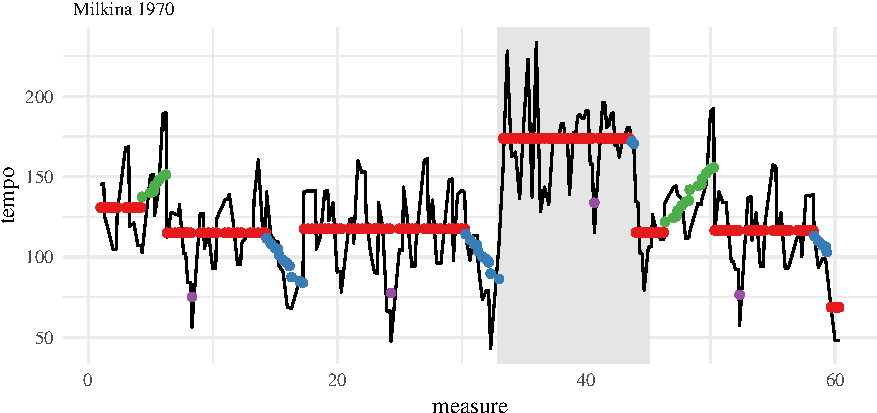
\includegraphics[width=\textwidth]{figs-for-paper_files/figure-latex/first-performance-1.pdf}
    \caption{Fliere's 1977 performance. The black line is what was played, while the dots represent our fit of the intended tempo.}
    \label{figure:fliere}
\end{figure}

For Yakov Fliere's 1977 recording of Chopin's Mazurka Op. 68 No. 3, our model produced parameter estimates shown in \ref{table:fliere}. This means that our model estimates Fliere's variance around his intended tempo to be 49 beats per minute, ???????????, the average magnitude of his acceleration or deceleration to be 25 beats per minute per measure, the average amount by which he slows down when emphasizing a note to be 32 beats per minute, the variance of his accelerations and decelerations to be 517, ???(question about $\mu$)???, and ???(modify figure 3?)???.

\begin{table}[]
\begin{tabular}{lllllllllll}
$\sigma_\epsilon^2$ & $\mu$????? & $\tau$ & $\varphi$ & $\sigma_2^2$ & $\sigma_3^2$ & $\sigma_4^2$ & $p_1$ & $p_2$ & $p_3$ & $p_4$ \\
927 & 174 & -23 & -30 & 433 & 976 & 398 & 0.95 & 0.02 & 0.64 & 0.58\\
\end{tabular}
\caption{parameter estimates for Tomsic's performance}
\label{table:tomsic}
\end{table}

\begin{figure}
    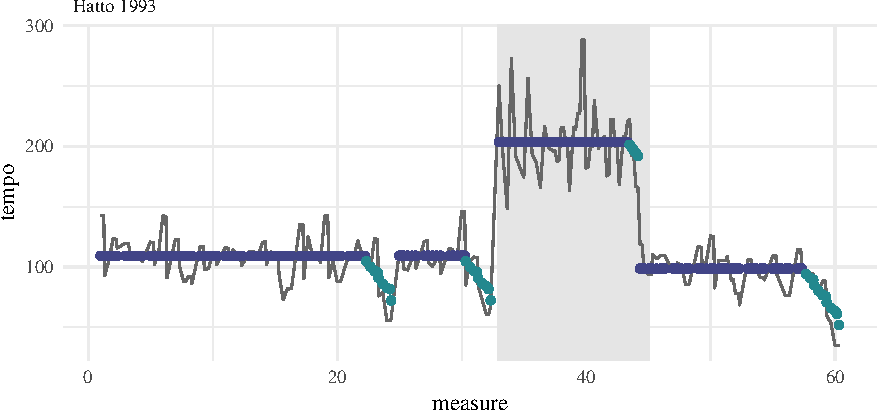
\includegraphics[width=\textwidth]{figs-for-paper_files/figure-latex/second-performance-1.pdf}
    \caption{Tomsic's 1995 performance. The black line is what was played, while the dots represent our fit of the intended tempo.}
    \label{figure:tomsic}
\end{figure}

We can see that our model's parameters have very simple musical interpretations. By looking at the estimates produced by fitting our model we can make comparisons between different performances. For example, we can compare Fliere's performance with Tomsic's 1995 performance. The estimates of the parameters for Tomsic's performance are provided in \ref{table:tomsic}.

\section{Discussion}




\bigskip
\begin{center}
{\large\bf SUPPLEMENTARY MATERIAL}
\end{center}

\begin{description}

\item[R-package ``dpf'':] R-package containing code to perform the
  methods described in the article. The package also contains all data
  sets used as examples in the article. (GNU zipped tar)

\end{description}




\bibliographystyle{agsm}
\bibliography{AllReferences}
\end{document}
